\documentclass[12pt]{article}
\usepackage{graphicx} % Required for inserting images
\usepackage[table]{xcolor}
\usepackage{tcolorbox}
\usepackage{hyperref} % For hyperlinks
\usepackage[a4paper, margin=1in]{geometry}
\usepackage{fancyhdr}
\usepackage{ragged2e}
\usepackage{subcaption}
\usepackage{natbib}



\pagestyle{fancy}
\fancyhf{}  % Clear default header/footer

% Customize header
\fancyhead[R]{\textbf{Student Id: 23189618}}  % Left header: Student ID




\fancyfoot[C]{\thepage}  % Footer: Centered page number

% Ensure the header width matches the body text width
\renewcommand{\headwidth}{\textwidth}  % Match header width to body text

\begin{document}

% First page content
\begin{titlepage}
    \centering 
   
    % Include the image
    
\includegraphics[width=1.1\textwidth]{BCU-logo.jpg} \\[3cm] % Adjust the width and path as necessary
    
    % Title
    {\Large \textbf{Data Visualization Assessment}} \\[1cm]
    
    % Author information
    \textbf{Bibek Sapkota} \\
    Student ID: 23189618 \\[0.2cm]

    Total Page Count: 37 \\[0.5cm]
    
    % Date
    \textbf{October 2024}
    
\end{titlepage}




\newpage % This will start a new page
\tableofcontents % To generate table of contents
\newpage
\listoffigures % Generates the List of Figures
\newpage


\begin{center}

    \LARGE \textbf{Visualization of Patterns in Thyroid Disease Progression: A Data-Driven Analysis}
\end{center}

\vspace{0.2cm}

\section{Introduction}

\vspace{0.2cm}

\subsection{Thyroid Function}
The thyroid gland is essential for human health, and thyroid dysfunction is particularly common in regions with iodine deficiency, given vital role in hormone production  \citep{Arthur&Beckett} .
It plays a pivotal role in regulating essential bodily functions, including metabolism, growth, and development. A thyroid nodule is a discrete lesion within the thyroid gland that is radiologically distinct from the surrounding thyroid parenchyma \citep{Cooper} .
More than 90\% of detected thyroid nodules are clinically insignificant because they have no ultrasound features that suggest malignancy or because they are cytologically benign \citep{Durante} .
When thyroid function is impaired, it can lead to conditions such as hypothyroidism, hyperthyroidism, or thyroid cancer, each presenting distinct challenges for patient health. % Understanding the mechanisms by which these disorders arise and progress is critical for devising effective medical interventions and managing patients. 
Analyzing these dysfunctions offers valuable insights that can guide early diagnosis, targeted treatments, and personalized patient care strategies.



\subsection{Motivation  behind the chosen domain}
Globally, the prevalence of thyroid cancer is still rising , with  with \emph{differentiated thyroid cancer }  being the most frequent type, accounting for about 95\% of cases \citep{cabanillas2016} and it's crucial to understand the factors that affect patient outcomes, As This trend makes knowledge of the elements affecting patient outcomes even more urgent. Clinical data analysis informs treatment and care for patients by highlighting more effective therapeutic approaches and refinement of prevention. It might also lead to a better understanding of the natural history of a disease and of its interaction with patient-specific variables, hence allowing personalized medicine approaches that tailor treatments to individual needs.


\subsection{Scope of the visualizations}
Visualizations in this report are geared toward the discovery of important patterns and insights in data on thyroid disease outcomes, recurrence, and treatment. The analytic investigation will consider a broad range of variables, from demographic and lifestyle factors to clinical attributes, in describing the complex nature of thyroid disease. The following relationships shall be visually analyzed to inform improvements in medical decision-making and management of the patient. A set of key questions about the dataset are answered using the visualizations:

\begin{itemize}
\item \textbf{Demographic Analysis}: To illustrate the mapping of the distribution of thyroid diseases according to age groups and sex, which will describe the trend of thyroid disorders in onset and development. This will indicate whether any particular demographic group is more prone to thyroid dysfunction or thyroid cancer.

\item \textbf{Lifestyle Factors and Thyroid Diseases}: Assessing the impact of lifestyle factors, such as smoking history and history of radiotherapy on thyroid function and the course of cancer. It will further be visually portrayed in comparing the severities of thyroid conditions amongst patients of different statuses of smoking and with or without a history of radiotherapy.

\item \textbf{Thyroid Status and Stage of Cancer}: Analyzing the association of thyroid status with stage of cancer. It would be seen from the plots the distribution of the staging where patients with normal thyroid status-euthyroid-are more likely to be diagnosed in the earlier stages, while abnormalities in thyroid status are associated with the advanced stages of the disease.

\item \textbf{Recurrence Rate and Risk Factors}: Analyzing recurrence rates in thyroid malignancy regarding demographic, clinical, and lifestyle factors. The plots illustrate variation in cancer recurrence rates according to sex, age group, adenopathy, and pathology type.

\item \textbf{Treatment Outcome by Demographics and Stage of Cancer}: It demographically maps the patient's age and gender with response to treatments regarding thyroid disorders. This would also include treatment success rate analysis across different age groups and stages of cancer, which can help identify the most responsive group toward the treatment.

\item \textbf{Treatment Response Modulated by Smoking}: Investigating the role of smoking status in modifying treatment responses at different stages of cancer. Visualizations will show how differences in treatment efficacies between smokers versus nonsmokers are varied, especially in early versus advanced stages of thyroid cancer.

\item \textbf{Physical Examination Findings and Levels of Risk}: Findings from physical examinations, such as nodules or goitres, are charted against the levels of risk that the patients have been categorized into. This will then help in identifying whether certain physical examination findings are indeed more indicative of a high-risk thyroid disorder.

\item \textbf{Feature Correlations}: Visualize the correlation of numeric features such as thyroid function, pathology type, and tumor size. These plots will show the significant correlation that can be useful in modeling thyroid cancer outcomes or understanding disease progression.
\end{itemize}

%\subsection{Dataset and Libraries Used}
% The dataset(Thyroid\_Diff.csv) used to perform this analysis consists of a large number of patients, where thyroid functions, demographic information, and treatment responses are included. Major libraries in R that allow cleaning, transformation, and visualization of data include ggplot2, dplyr, tidyverse and plotly which can manipulate and graphically represent data at an advanced level with much accuracy and comprehensiveness within the dataset.

\subsection{Aims and Objectives}
This analysis essentially focuses on the understanding, through visualization, of various factors related to the progression, recurrence, and treatment outcomes in thyroid disease, using comprehensive patient data. The study shall try to elucidate how patient demographics, lifestyle factors, thyroid function, and clinical outcomes are interrelated by tapping into data-driven insights. This is ultimately to support diagnosis, treatment planning, and improved strategies for patient management of thyroid disorders.
\newpage

\textbf{ Objectives of Visualization}
\begin{itemize}

    \item \textbf{ Demographic pattern analysis:}: Demographic pattern analysis means how thyroid disorder varies across age group and gender; and what significant trends, if any, can be traced about the onset, progression, recurrence, and staging of the disease.

\item \textbf{ Life-course factors analysis}: What history of smoking and radiotherapy treatment effects does lifestyle have on the stage of thyroid disease and possible recurrence?.

\item \textbf{ Explore thyroid function}: Visualize the distribution of thyroid status with regard to thyroid function (euthyroid, hypothyroid, and hyperthyroid) against cancer stage and physical examination findings.

\item \textbf{ Treatment outcome comparison}: Assess treatment response rates of various treatments stratified for patients' demographic data, stages of cancer, and categories of thyroid function, underlining treatment response and recurrence rates.

\item \textbf{ Clinical feature correlation}: Explain the correlation of the clinical features, such as adenopathy and stages of cancer, which would relate to the outcomes and recurrence rates in the patient.

\item \textbf{ Identifying high-risk groups}: Highlight specific risk factors and demographic groups that may be more prone to recurrence or unsatisfactory treatment outcomes; this would prove useful for actionable insights on personalized treatment approaches.
\end{itemize}

\newpage 


\section{Data Exploration}

\subsection{About the dataset}
This dataset covers the prevalence and attributes of thyroid conditions in a given patient population, with data analyzed against a broad set of demographic, past medical history, and clinical outcome variables. In this database, the key attributes have been included that could be useful in understanding disease progression and response to treatments in thyroid disorders. Each record offers very valuable insights into the condition of the patient and the efficacy of treatment given, and can thus be analyzed for an improved diagnosis and therapeutic intervention in thyroid health.
\vspace{0.5cm}

\textbf{Column Descriptions:}

\begin{itemize}
\item \textbf{Age}: The age of the patient at the time of diagnosis in years.
    \item \textbf{Gender}: The gender of the patient, recorded as male (M) or female (F).
    \item \textbf{Smoking}: Indicates whether a patient is currently a smoker or not.
    \item \textbf{Hx Smoking}: History of smoking; yes/no indicating whether the patient has smoked in the past.
    \item \textbf{Hx Radiotherapy}: History of undergoing radiotherapy treatment (Yes/No).
    \item \textbf{Thyroid Function}:Indicates current status of the patient's thyroid function.
    \item \textbf{Physical Examination}: Results from physical examination of the thyroid.
    \item \textbf{Adenopathy}: Indicates whether adenopathy (swollen glands) was present (Yes/No).
    \item \textbf{Pathology}: The type of pathology identified from tissue samples. 
    \item \textbf{Focality}: Whether the tumor is uni-focal(single) or multi-focal(multiple).
    \item \textbf{Risk}: The risk classification assigned to the patient.
    \item \textbf{T}: The T classification indicates tumor size.
    \item \textbf{N}: The N classification indicates the level of lymph node.
    \item \textbf{M}: The M classification indicates whether metastasis (spread of cancer to other parts of the body) has occurred.
    \item \textbf{Stage}: The overall cancer stage based on the TNM classifications, ranging from Stage I to Stage IV.
    \item \textbf{Response}: The patient's response to treatment, including whether the disease has stabilized, improved, or worsened.
    \item \textbf{Recurred}: Indicates whether the cancer has recurred after thetreatment (Yes/No).
\end{itemize}



\subsection{Missing Values}
I used R's colSums() function in combination with is.na() to determine which missing values were in the data set. ColSums() effectively counts the number of null entries in a given column. This will display systematic results using print(missing\_values) and provide an exact count of the number of missing values within a column.

\begin{figure}[h]
    \centering
    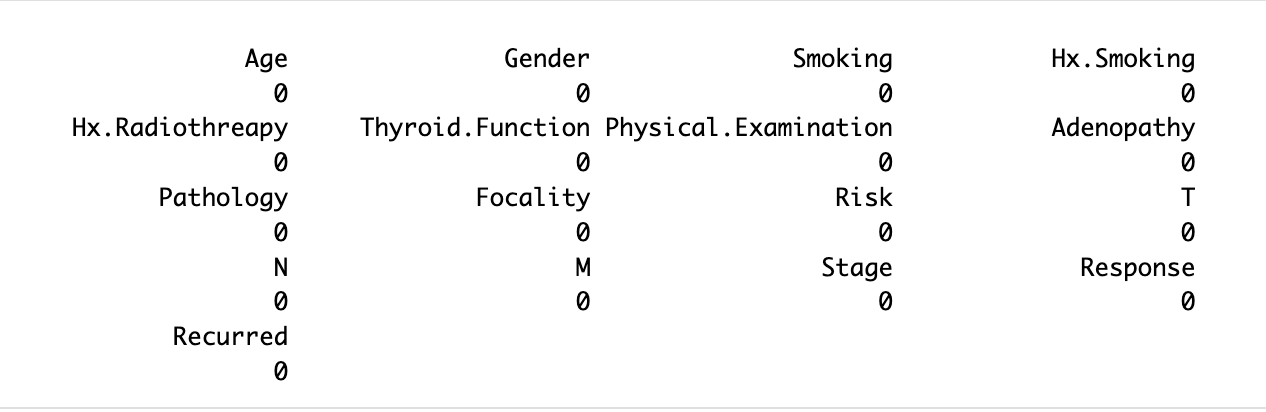
\includegraphics[width=1\textwidth]{Missing.png}  
    \caption{Number of Missing Values per Column}
        \label{fig:example}
   \vspace{0.5cm}
\end{figure}
     
\justifying As show in above figure there are  zero counts in every column, the analysis verified that there were no missing values at all. This result guarantees that no data imputation techniques are required because the dataset is fully populated and is prepared for additional analysis.

\subsection{Duplicate Values}
In cleaning the data set for analysis , we determined there were duplicate records. We found nineteen duplicate rows using the duplicated() function, which goes through every row across columns and flags the repetition. We then used the addition of these duplicates with sum(duplicates) to count how many are in order to show the duplicate rows.

\begin{figure}[h]
    \centering
    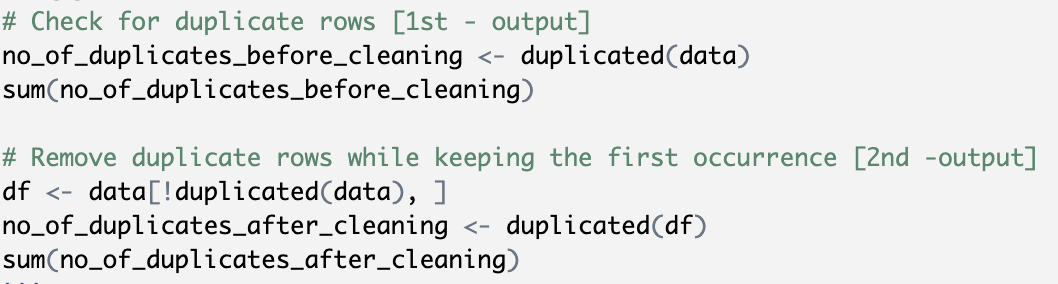
\includegraphics[width=1\textwidth]{Duplicate.png}  
        \label{fig:example}
   \vspace{0cm}
\end{figure}

These duplicates were cleared for the integrity and cleanliness of our data. The negated output of this function, duplicated(), filtered out the repeats in the dataset and retained only the first occurrence. We reassessed the cleaned dataset to confirm that the duplicates had been removed and checked the new row count by using print(nrow(df)). This is a very important step in keeping our data intact, meaning it gives reasons on which we may base our conclusions that are unique and not redundant.

\newpage


\section{Feature Engineering}
A new feature called "Smoking\_Status" was created in the dataset development process to provide more information on the impact of smoking habits on health outcomes. Two previous columns— 'Smoking' and 'Hx.Smoking' that represented smoking behaviors in the past and present, respectively, were combined to create this feature. \\ [0.3cm]
\textbf{process: }

The "Smoking\_Status" column was created using the R package dplyr and the following criteria:
\begin{enumerate}
    \item \textbf{Ever Smoked}:  Subjects fall under this category depending on whether they smoke or has smoke in past. The 'Ever Smoked' in the column against smoking\_status indicates that persons either smoke now or have smoked in the past.
    \item \textbf{Never Smoked}: In the absence of a 'Yes' in either column (Smoking and Hx.Smoking), the status given would be "Never Smoked," and that person never smoked.
\end{enumerate}

\begin{figure}[h]
    \centering
    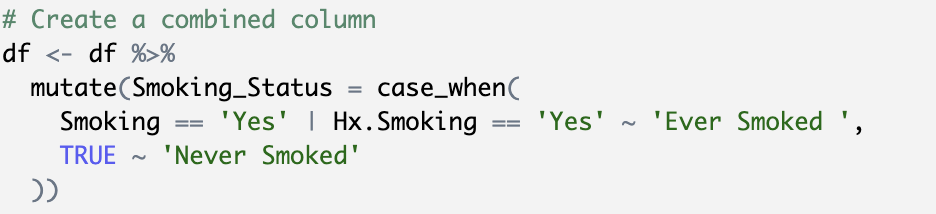
\includegraphics[width=1.03\textwidth]{feature enge.png}  
        \label{fig:example}
   \vspace{0cm}
\end{figure}

\textbf{Justification: }
\begin{enumerate}
    \item \textbf{Simplifying Data for EDA:} Such a combination of variables into one feature is a simplification of the data. This simplification allows the analyst to conduct EDA more simply; hence, finding trends and patterns related to smoking habits and health outcomes corresponding to those habits is efficient.
    \item \textbf{Enhancing Analytical Accuracy:}  This combination of feature will make the dataset more beneficial for EDA, as it explains the variable of any smoking exposure, whether past or present. Usually, the current and past practices of smoking are high-value factors when research analysis of such kind needs correct judgments about health hazards and outcomes.
\end{enumerate}

This feature engineering effort not only simplifies the dataset for more effective EDA but also enhances the ability to uncover meaningful insights into how smoking behaviors influence health.
\newpage


\section{Data Visualization}

\subsection{Answering the questions through data visualization} 
This section is supported by a thorough research design in which each
question was answered with due preparation . The answers are allowed to
ensure that clear and detailed understanding, as well as insights into the
problem, are clearly explained.Relevant graphics are included to the facts
presented to enhance this understanding and complement the review and
presentation for the purpose of better organization. This will ensure that the findings of the research will actually meet the objective of the presentation,wherein the text will support the pictures and vice versa. As well as expectation, which is also mentioned as 'E', represents an expectation for the question.

\subsubsection{Demographic Analysis}

\begin{enumerate}
    \item \textbf{How does age distribution and Gender distribution vary among different thyroid function categories ?}\\
    E: It is expected that the older the patients are, the faster the stage of thyroid cancer. Whereas, Gender is not expected to have a significant impact.

    
    
    \begin{figure}[h]
        \centering
        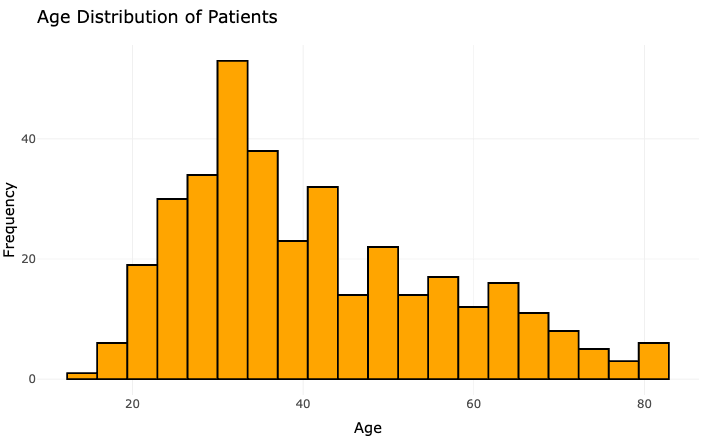
\includegraphics[width=1\textwidth]{age dist.png}  
        \caption{Age Distribution of Patients}
            \label{fig:figure2}
       \vspace{0cm}
    \end{figure}

The age distribution of thyroid patients is clearly dominated in the younger to middle-aged population, with the majority of the cases occurring at an age of about 35 years. After this peak, the number of the patients gradually decreases, with much fewer scenarios found in people over 60. It would thus appear that though thyroid conditions are more common among young adults, it can occur at any age.


\hspace{9pt} Whereas a distinct overlap in age groups suggests that the occurrence of thyroid issues is not heavily biased toward any specific age group. In many cases, thyroid nodules may be detected because of their size or anterior position , or the skill of the physician performing the examination \citep{Vanderpump} .

 
 \begin{figure}[h]
 \vspace{25pt}
        \centering
        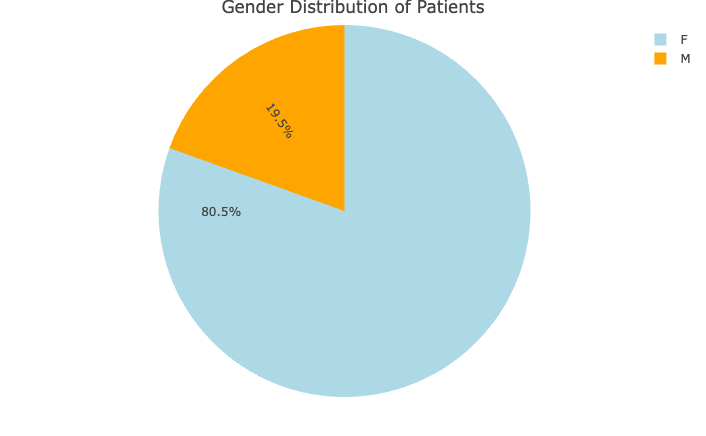
\includegraphics[width=1\textwidth]{Gender Dist.png}  
        \caption{Gender Distribution of Patients}
            \label{fig:example}
       \vspace{0.5cm}
    \end{figure}

The above chart on the gender distribution of patients clearly indicates an overwhelming dominance by female patients in relation to male patients. It is indicated that 80.5\% of the patients are females, abbreviated as F, while those referred to as males, abbreviated as M, constitute 19.5\%. This reveals great disparity in distribution and may indicate that thyroid conditions could be more prevalent in women than in males. These kinds of trends could be contributed to by biological, hormonal, or genetic predispositions which make females susceptible to thyroid conditions.


\hspace{9pt} Despite the fact that both genders are affected by thyroid conditions, the skewed distribution does not appear to show this. The fact that almost 20\% of the patients are males drives home the message that,  Thyroid diseases are widespread conditions, occurring significantly more often in females than in males \citep{Bauer} .

\newpage

 \begin{figure}[h]
 \vspace{25pt}
        \centering
        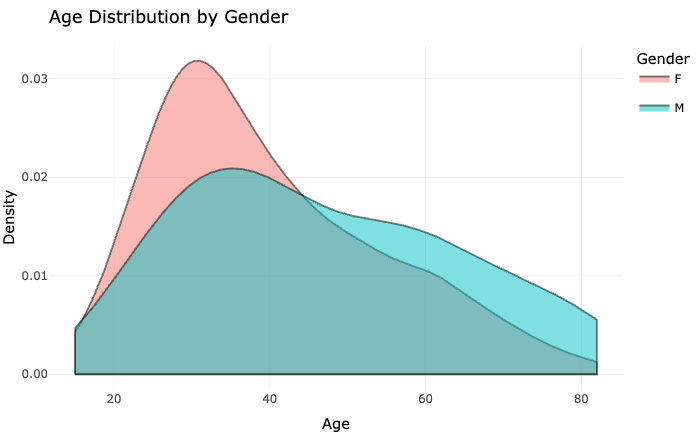
\includegraphics[width=1.15\textwidth]{age vs gender.png}  
        \caption{Age Distribution by Gender}
            \label{fig:example}
       \vspace{0.5cm}
    \end{figure}

The density plot shows the Age distribution by gender for thyroid conditions., it will show age demographics overlay between male and female patients diagnosed with thyroid conditions. From this plot, the two genders are very similar in age profile-the majority of the cases fall within the young to middle-aged groups. The peak in both sexes happens in the mid-thirties, which insinuates that thyroid conditions are most prevalent in this age bracket. A density plot showing a wider spread in females indicates that age of prevalence is wider than in males, whose age distribution appears slightly narrowed.

While the overall trend is towards younger to middle-aged patients, the plot shows that thyroid conditions can happen at any age, hence not being confined to any particular group of patients. The graph further suggests that thyroid conditions indeed have a higher prevalence among females, as suggested by the gender distribution showing the majority of patients to be females. It is also important to emphasize that age distributions overlap in gender, thus reinforcing the notion of higher preponderance in females and a wide age group affected in both males and females; thus, most demographic groups are affected by thyroid disorders.
\newpage

\item \textbf{What are the statistical correlations between age,gender and recurrence rates in thyroid patients?}\\ [5pt]
    E:Recurrence rates may be lower in younger than in older patients, and it is expected that recurrence rates could be higher in females compared to males .

 \begin{figure}[h]
 \vspace{5pt}
        \centering
        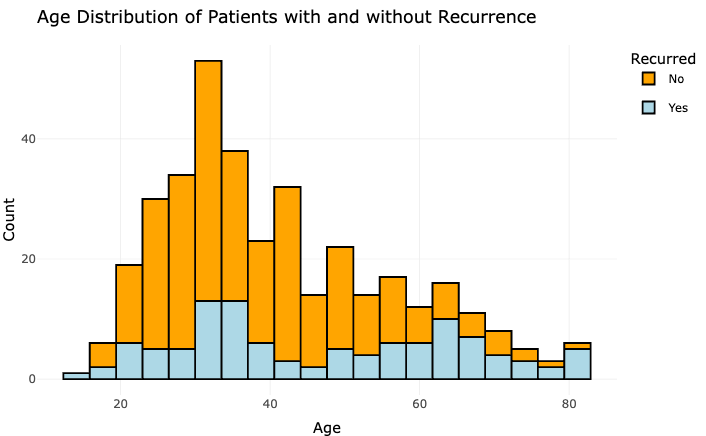
\includegraphics[width=1.1\textwidth]{Age vs recurrence.png}  
        \caption{Recurrence rate in different age}
            \label{fig:example}
       \vspace{1cm}
    \end{figure}


The age distribution of thyroid patients is clearly dominated in the younger group to middle-aged population, as shown in (Figure~\ref{fig:figure2}) with significant concentration of cases around age 35. Recurrence is observed in all age groups; however, no overwhelming bias in any particular age group exists. Though the overall representation seems to be more for the younger patients, recurrence doesn't appear to increase significantly with age or become more frequent in older individuals.

\hspace{9pt} This suggests that, while age may not be the strongest predictor of recurrence, further statistical tests might be needed to identify subtle trends in older or younger patients, especially when other risk factors are considered.

\newpage

    \begin{figure}[h]
        \vspace{5pt}
        \centering
        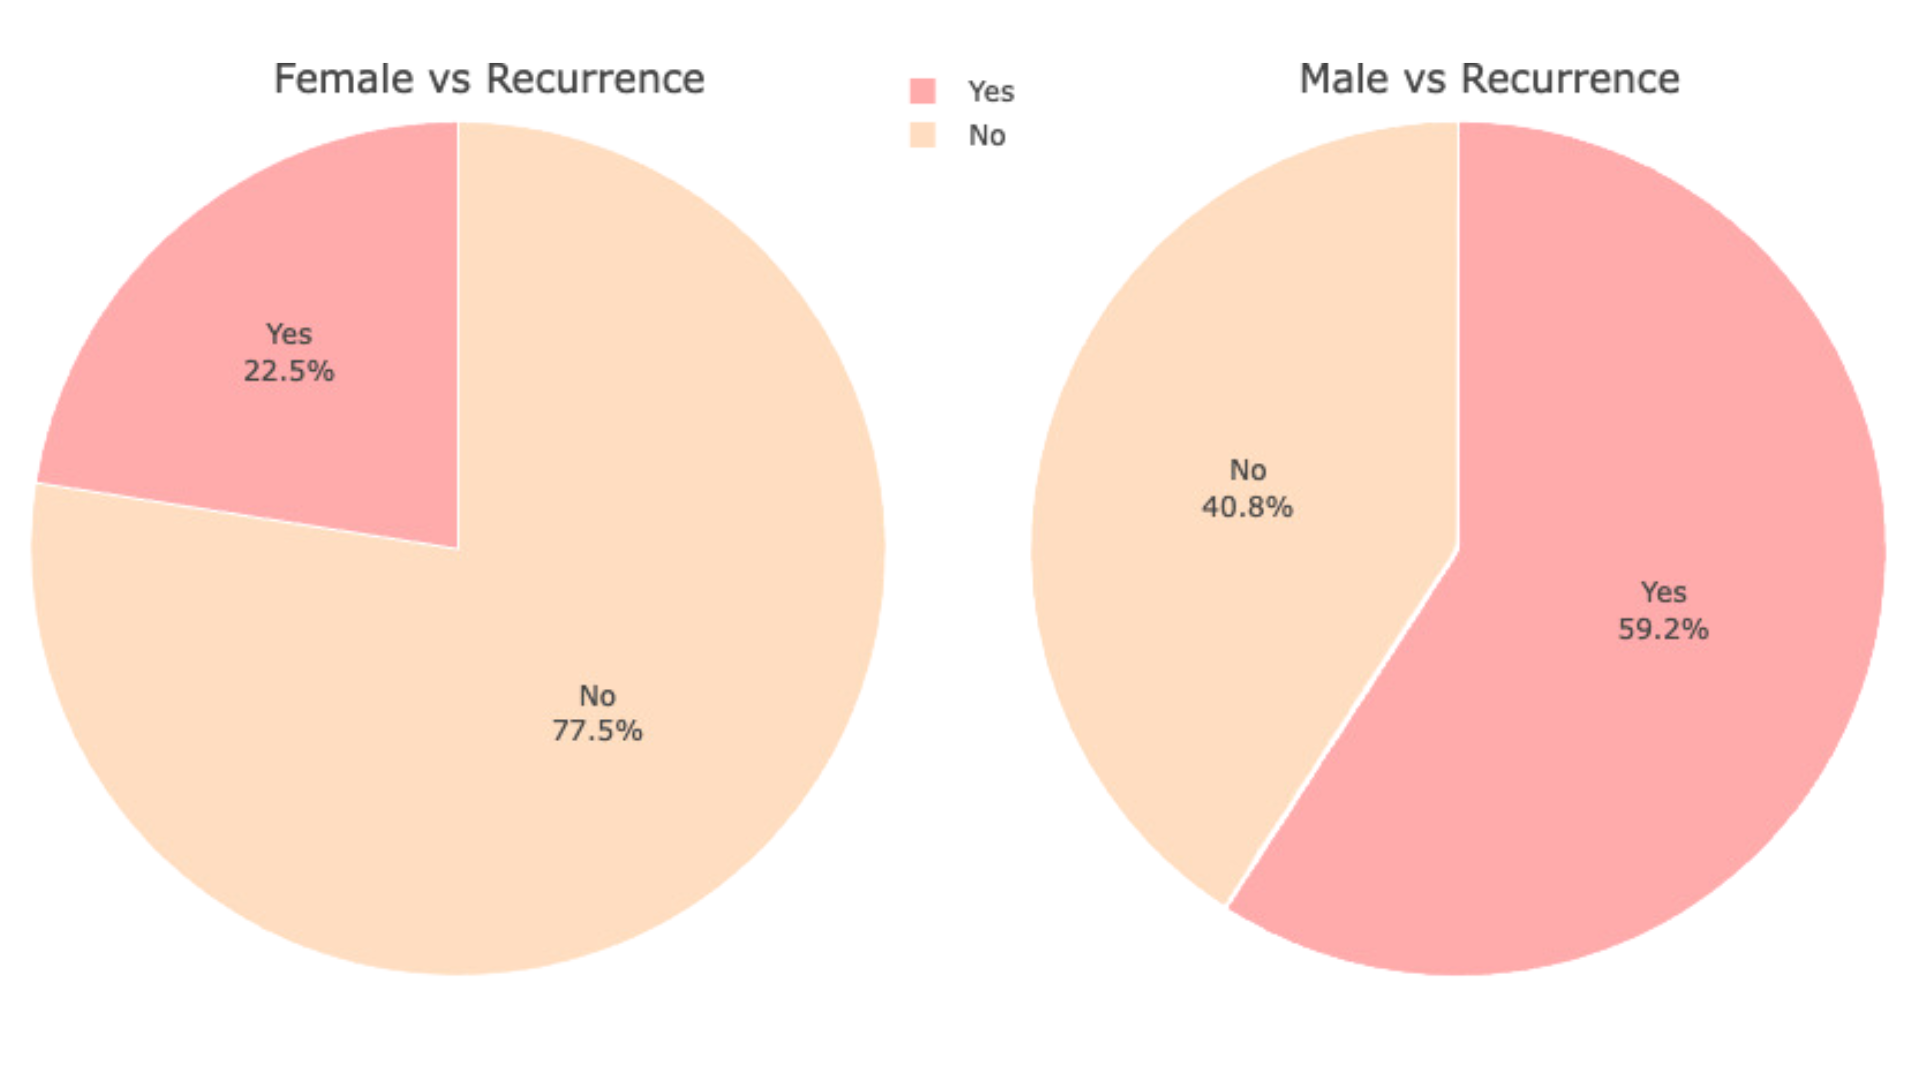
\includegraphics[width=1\textwidth]{gender vs recurrence.png}  
        \caption{Recurrence rate comparison by gender}
            \label{fig:example}
       \vspace{1cm}
    \end{figure}

These two pie charts show sharp contrasts in the gender distribution according to recurrence status among thyroid patients. Only 22.5\% of the female patients went into recurrence, while the majority- 77.5\% of the female patients did not face recurrence. This indicates that the larger proportion of female patients has maintained a stable outcome after receiving treatment. In contrast, the male patients exhibit a significantly higher recurrence rate- 59.2\% of the patients suffered recurrence, whereas 40.8\% did not. This higher recurrence rate in males would therefore be indicative of greater risk for this group concerning thyroid cancer outcome.

\hspace{9pt} This might mean that the male patients are more vulnerable to recurrence of thyroid cancer compared to females. That a gap exists between the genders adds to curiosity on what possibly could contribute to such an outcome, which might include biological factors or environmental exposures, or differences in treatment received
\newpage

\end{enumerate}

\newpage

\subsubsection{Lifestyle and History Factor}

\begin{enumerate}
    \item \textbf{Does smoking correlate with the severity of thyroid pathology findings?} \\ [4pt]
    E: Those patients with smoking may show more aggressive pathology, a reflection of the deleterious effects of tobacco on the thyroid gland.

 \begin{figure}[h]
        \vspace{5pt}
        \centering
        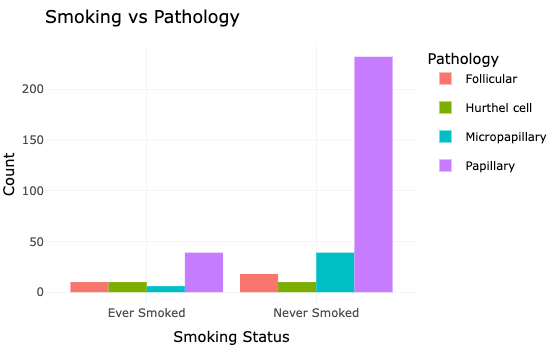
\includegraphics[width=1.1\textwidth]{smoking vs pathology.png}  
        \caption{Smoking status and severity of thyroid pathology}
            \label{fig:example}
       \vspace{0.5cm}
    \end{figure}

The above plot illustrates the clear predominance of "Never Smoked" patients in the category of Papillary pathology while the other pathologies, namely Follicular, Hurthel cell, and Micropapillary, are less well-represented across both "Ever Smoked" and "Never Smoked" groups. There is no overwhelming relationship that would appear to exist between smoking history and the severity of thyroid pathology, because "Ever Smoked" does not seem to have more serious or different pathologies compared to non-smokers.

\hspace{9pt} This may indicate that smoking status is not a very powerful predictor of specific types of thyroid pathology; at least in one of the most common-thyroid cancers-papillary thyroid cancer, it does not appear to be linked with smoking history.

\newpage

   \item \textbf{Are there differences in cancer stages between current smokers and those with a history of smoking? } \\
   E:Current smokers are expected to found to have more advanced cancer stages compared to those with a history of smoking.

 \begin{figure}[h]
        \vspace{5pt}
        \centering
        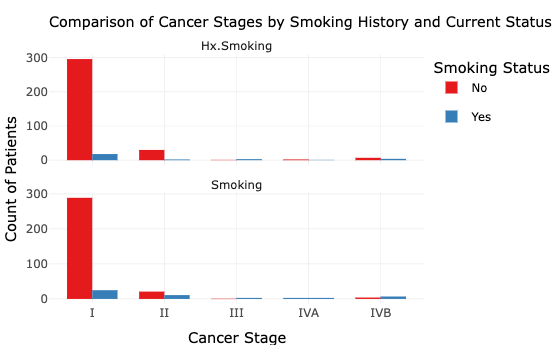
\includegraphics[width=1.1\textwidth]{smoking all.png}  
        \caption{Cancer Stage by Smoking History and Current Status}
            \label{fig:example}
       \vspace{0.5cm}
    \end{figure}

This bar chart illustrate the distribution of tumor cancer stages among patients with or without a history of smoking and current smokers. Indeed, it gives a different trend for five stages, such as I, II, III, IVA, and IVB. Most patients with a history of smoking were diagnosed at earlier stages, while the numbers decreased considerably through the later stages, showing an earlier stage of diagnosis in former smokers. At all stages, the current smokers are highly sparse, with just a couple of patients in each category; this may indicate that either the sample size is smaller or the trends show that current smokers are diagnosed less often or even later in stages due to late seeking of health care or symptom recognition. This disparity in stage distribution suggests a differential timing of detection of cancers or access to health care between former and current smokers and therefore suggests the possible need for more active health monitoring with earlier intervention for current smokers.
\newpage


       \item \textbf{What impact does previous radiotherapy have on current thyroid function status?}\\
E: Previous radiotherapy can negatively impact current thyroid function, often leading to hypothyroidism or other thyroid dysfunctions due to radiation-induced damage to the thyroid gland

        \begin{figure}[h]
        \vspace{5pt}
        \centering
        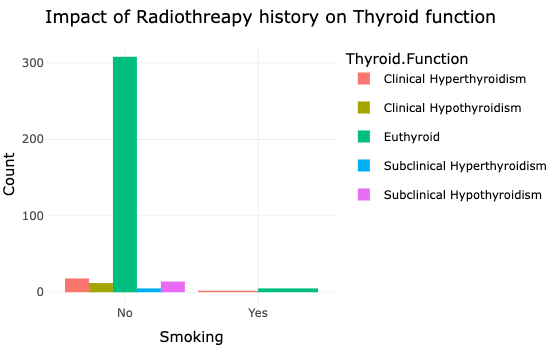
\includegraphics[width=1.1\textwidth]{radio with thy.png}  
        \caption{Radiothreapy history on Thyroid Function}
            \label{fig:example}
       \vspace{0.5cm}
    \end{figure}

The graph demonstrates that, among the cases with no radiotherapy history, the majority of cases were found to be Euthyroid, or of normal thyroid functioning status. In contrast, those experiencing radiotherapy show a greater distribution across various thyroid statuses such as Clinical Hypothyroidism, Clinical Hyperthyroidism, and Subclinical Hypothyroidism.

\hspace{9pt}  This pattern shows that most of the patients with no history of radiotherapy are normal, while most of those with a history of radiotherapy might predispose them to thyroid dysfunction.

 

\newpage

       \item \textbf{How does radiotherapy history affect the risk of thyroid cancer recurrence?} \\
       E: A history of radiotherapy increases the risk of thyroid cancer recurrence, as radiation exposure can contribute to long-term thyroid gland damage

        \begin{figure}[h]
        \vspace{5pt}
        \centering
        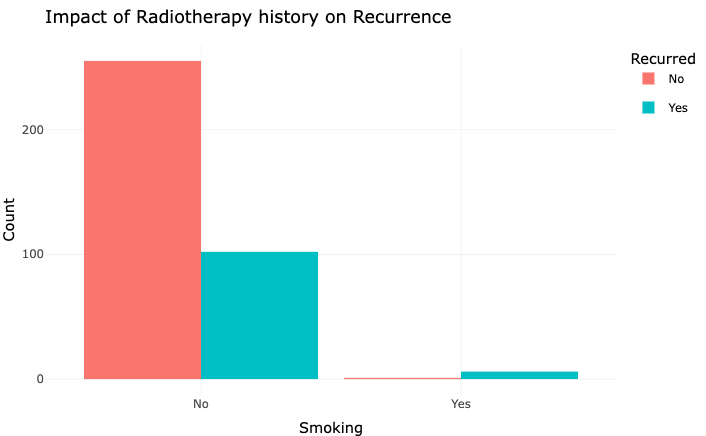
\includegraphics[width=1.1\textwidth]{radio and reccure.png}  
        \caption{Impact of Radiotherapy history on Recurrence}
            \label{fig:example}
       \vspace{0.5cm}
    \end{figure}

This graph illustrates that patients without a history of radiotherapy had the most frequent rate, although there is a disproportionate percentage who experienced recurrence. In contrast, the patients who have a history of radiotherapy are at an overall count far lower but where the recurrence is more equally distributed, having a slight increase in cases where there was a recurrence compared to ones that did not experience it.\\ 



\hspace{9pt} It shows that radiotherapy does not ensure the recurrence of thyroid cancer, but in patients with a previous history of radiotherapy, there is a slight increase. The overall recurrence rate is higher in radiotherapy patients compared to non-radiotherapy patients. 

\end{enumerate}
\newpage

\subsubsection{Medical Analysis}

\begin{enumerate}
    \item \textbf{Which thyroid function is most prevalent ?}

 \begin{figure}[h]
        \vspace{5pt}
        \centering
        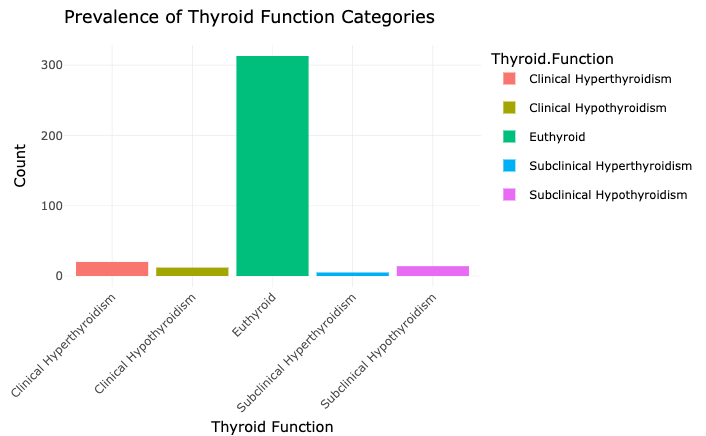
\includegraphics[width=1.15\textwidth]{prevelence vs function.png}  
        \caption{Distribution of Thyroid Function}
            \label{fig:example}
       \vspace{0.5cm}
    \end{figure}

The above graph shows that most of the people fall into the category of Euthyroid, which means normal thyroid function. The rest of the categories of thyroid function include Clinical Hyperthyroidism, Clinical Hypothyroidism, Subclinical Hyperthyroidism, and Subclinical Hypothyroidism, and they have very negligible counts. This can be interpreted to mean that thyroid dysfunction is way less common when compared to normal thyroid function in the population under study.

Thyroid disease affects cardiovascular function significantly, altering cardiac output, contractility, blood pressure, and systemic vascular resistance, making early detection critical for preventing associated complications."

\hspace{9pt} This therefore suggests that the normal functioning of the thyroid is the prevailing thyroid status among the respondents; hence, the larger proportion is generally healthy in terms of their thyroid. On the contrary, the few thyroid dysfunctions recorded are truly a reflection of the presence of such conditions; however, these are quite rare.

\newpage


        \item \textbf{Is there a relationship between thyroid function and the physical examination findings ?}

 \begin{figure}[h]
        \vspace{5pt}
        \centering
        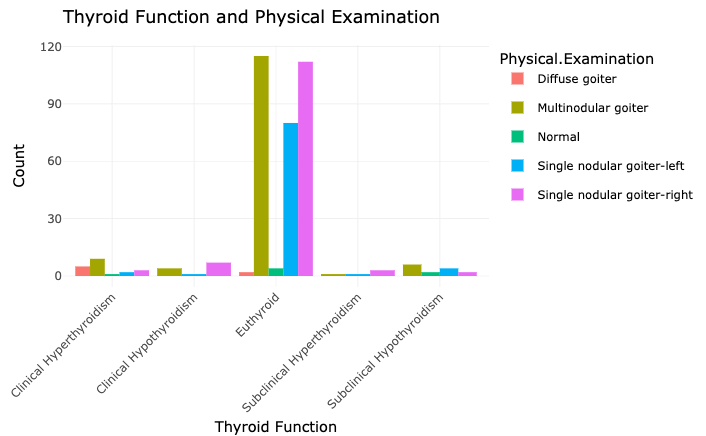
\includegraphics[width=1.15\textwidth]{thyroid and physical.png}  
        \caption{Realtionship of Thyroid Function and Physical Examination}
            \label{fig:example}
       \vspace{0.5cm}
    \end{figure}

    The above graph categorizes the patients based on thyroid function and then correlates these with the findings on physical examination. The majority of the patients fall under Euthyroid status, meaning normal thyroid status, and most of them do not usually have physical manifestations of thyroid problems, as can be seen in the high magenta bar under the normal category. This suggests that normally, a thyroid function that is normal is associated with a thyroid gland that is unremarkable on physical examination. At the same time, Clinical Hyperthyroidism and Clinical Hypothyroidism are significantly associated with diffuse and multinodular goiters, respectively, a fact indicated by the big yellow and green bars in these categories. 
    
    \hspace{9pt} This therefore shows  that thyroid dysfunction-both an overactive and underactive gland-is often physically manifested as several types of goiters.

\newpage

   \item \textbf{Do specific thyroid functions correlate with higher cancer stages at diagnosis ? } \\
   E: It is expected that the majority of euthyroid individuals are diagnosed at stage I of cancer, showing a significant concentration in the earliest stage of the disease. 

 \begin{figure}[h]
        \vspace{5pt}
        \centering
        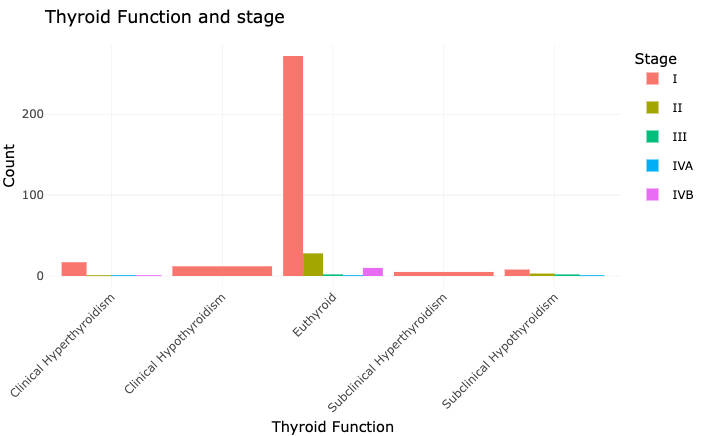
\includegraphics[width=1.15\textwidth]{thyroid vs stage.png}  
        \caption{Thyroid Function as comapred to Stage}
            \label{fig:example}
       \vspace{0.5cm}
    \end{figure}

The bar chart describes the distribution of different thyroid functions within various stages of cancer. The horizontal axis categorizes thyroid functions, while the vertical axis measures the number of cases identified in each stage of cancer. The most striking feature is the red bar under the Euthyroid category at stage I, reflecting that normal thyroid-function patients are mainly diagnosed at early stages, probably due to regular screening or a diagnosis at an early stage.

 \hspace{9pt} This graph also reflects minimal counts for other thyroid function categories across all cancer stages and has no significant peaks to show that specific thyroid dysfunctions have no direct relation to the diagnosis at more advanced stages of cancer. This absence of a trend is important in gathering insight into the implications brought about by thyroid health in understanding cancer progression and management.

\newpage

   \item \textbf{How does thyroid function vary with patient age and gender?} \\
   E: Thyroid function often changes with age and is more commonly problematic in women and older adults.

 \begin{figure}[h]
        \vspace{5pt}
        \centering
        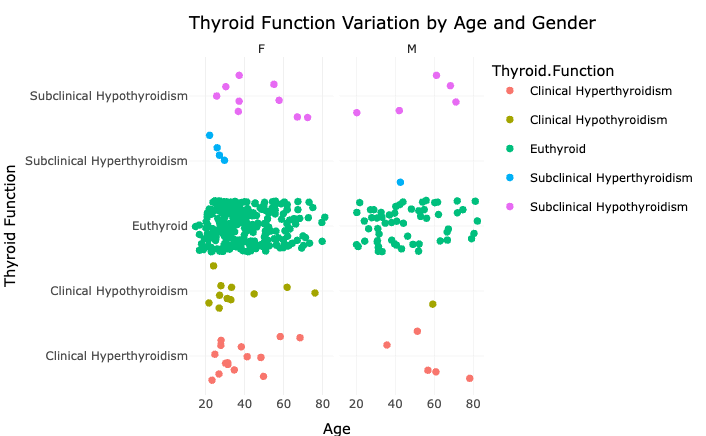
\includegraphics[width=1.15\textwidth]{thyroid vs age vs gender.png}  
        \caption{Thyroid Function by Age and Gender}
            \label{fig:example}
       \vspace{0.5cm}
    \end{figure}

The above scatter plot, "Thyroid Function Variation by Age and Gender", shows the overall thyroid function in the different age groups by gender. There is a big cluster of points in the category "Euthyroid" that encompasses pretty much most age brackets for both males and females. This reflects the fact that normal thyroid status is maintained across all ages, from young adults to the elderly. On the other hand, subclinical thyroid dysfunctions demonstrate mild female preponderance and a higher prevalence among younger and middle-aged women. Clinical Hyperthyroidism and Hypothyroidism conditions are relatively rare but with a very different pattern; most notably, Clinical Hypothyroidism is found more in older females, suggesting a vulnerability with age.

\newpage





\end{enumerate}

\subsubsection{Clinical Feature}

\begin{enumerate}


% \newpage

       \item \textbf{How does the presence of adenopathy correlate with thyroid cancer staging ?} \\
       E: The presence of adenopathy, can indicate a higher stage of thyroid cancer suggesting that the cancer may have spread beyond the thyroid gland.

 \begin{figure}[h]
        \vspace{5pt}
        \centering
        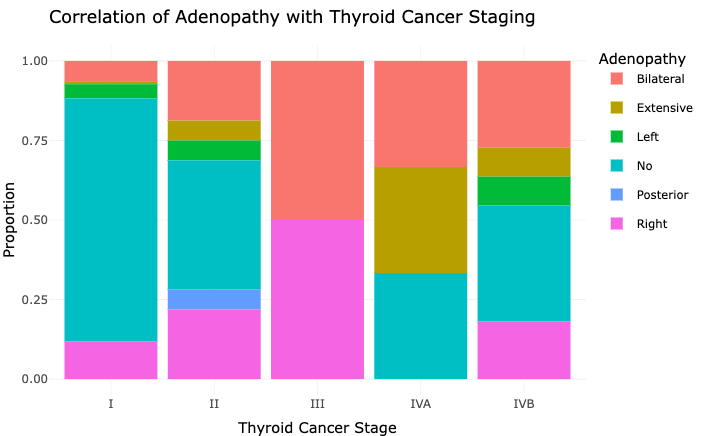
\includegraphics[width=1\textwidth]{adenopathy with satge.png}  
        \caption{Corelation of Thyroid stage and Adenopathy}
            \label{fig:example}
       \vspace{0.5cm}
    \end{figure}

    The following chart illustrates how the presence and type of adenopathy relate to various thyroid cancer stages. Note that the severity of adenopathy progresses with an increase in stage of cancer. For the earliest stages, I and II, most patients have no adenopathy, reflecting minimal lymphatic involvement. However, at Stage III, there is a drop in those cancer cases without adenopathy and an increase in those with extended adenopathy, showing wider lymph node involvement. During Stages IVA and IVB, the incidence of extended adenopathy becomes overwhelmingly greater, while the distribution of adenopathy itself becomes relatively even across different specific locations (left, right, bilateral, and posterior). 
    
    This would suggest that the lymphatic system in advanced stages of thyroid cancer is highly involved with the disease, indicating more aggressive disease that might broadly influence the approach to treatment. The trend underlines the possible utility of the extent of adenopathy as a clinical marker in assessing the stage and severity of thyroid cancer. 

\newpage


       \item \textbf{Do patients with adenopathy have higher recurrence rates compared to those without ?} \\
       E: Patients with adenopathy typically have higher recurrence rates of thyroid cancer than those without.

 \begin{figure}[h]
        \vspace{5pt}
        \centering
        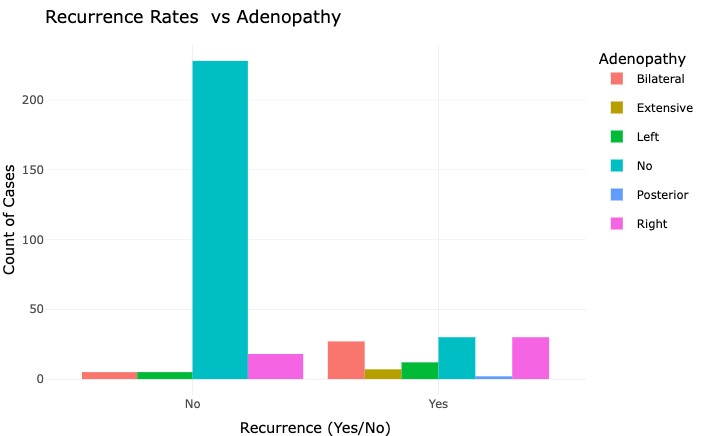
\includegraphics[width=1\textwidth]{recc vs adpt.png}  
        \caption{Recurrence Rate vs Adenopathy}
            \label{fig:example}
       \vspace{0.5cm}
    \end{figure}

This chart shows a bar plot on recurrence rates versus adenopathy in thyroid cancer patients, shows that the majority of those without adenopathy do not experience recurrence, meaning lower risk with the absence of lymph node involvement. In contrast, though the number of cases with adenopathy-whether to extensive, to both sides, the left side, the right side, or the posterior-is smaller, their presence is indicative of higher chances of recurrence. This would mean that the presence of adenopathy-a pointer to the more aggressive or extensive disease-considerably increases the possibility of recurrence and, therefore, requires serious follow-up with such patients.

Therefore, A definite trend within the data could be extracted that adenopathy of any kind is associated with an increased risk of recurrence. This can only mean that efficient lymph node management may hold the key to better long-term results. Thus, early detection and management of adenopathy during treatment planning may hold the key to minimizing risks of recurrence in thyroid cancer. 
    
\newpage 

 \item \textbf{What are the common physical examination findings across different risk categories ?} \\
 E: Common physical examination findings in thyroid cancer can vary by risk category: low-risk patients might have a small, whereas high-risk patients may present with multiple nodules.

 \begin{figure}[h]
        \centering
        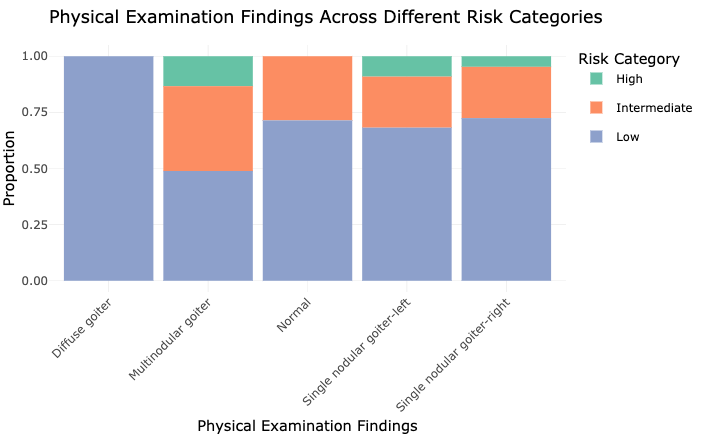
\includegraphics[width=1.1\textwidth]{physical vs risk.png}  
        \caption{Physical Examination vs Risk}
            \label{fig:example}
       \vspace{0.5cm}
    \end{figure}

The graph categorizes the findings of the physical examination into various risk levels of a medical condition. It defines the percentage distribution of low, intermediate, and high-risk observations. The findings listed are "Diffuse goiter," "Multinodular goiter," "Normal," "Single nodular goiter-left," and "Single nodular goiter-right." These categories are relatively evenly distributed across the three different risk categories for each finding type. Remarkably, the results of "Normal" are distributed across low, intermediate, and high risks in a relatively uniform distribution, which indicates that normal findings in themselves may not fully correspond to a low-risk category. Concerning "Single nodular goiter-left" and "Single nodular goiter-right," a similar pattern of patients' distribution has been observed, with a slight predominance of the former in the intermediate risk category, possibly reflecting a more nuanced interpretation of risk based on the nodular characteristics. The "Diffuse goiter" and "Multinodular goiter" are similarly well-represented, with a very good representation of the high-risk category-that is, these conditions are more likely to fall under higher medical risks. 

\end{enumerate}

\newpage

\subsubsection{Cancer-Specific Analysis}

\begin{enumerate}
    \item \textbf{How do demographic factors influence the distribution of TNM staging in thyroid cancer?} \\
    E: Demographic factors such as age, gender can influence the distribution of TNM staging in thyroid cancer, with younger patients often presenting with lower stages, while older adults might have more advanced stages at diagnosis. Gender differences also exist, with women typically diagnosed at earlier stages compared to men.
    
    \begin{figure}[h]
        \centering
        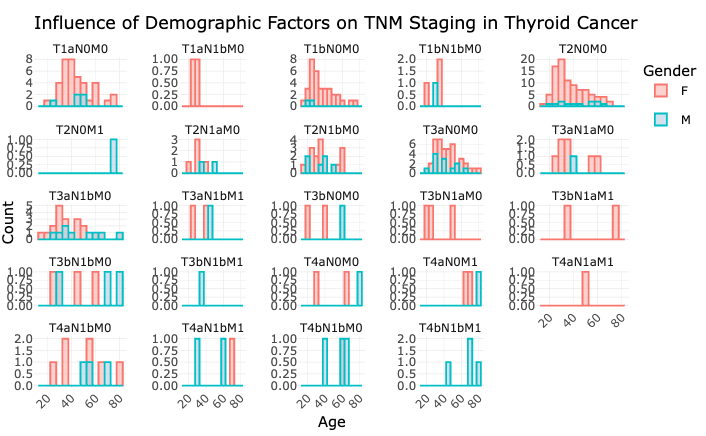
\includegraphics[width=1.1\textwidth]{demographic TNM.png}  
        \caption{Distribution of TNM staging in thyroid cancer}
            \label{fig:example}
       \vspace{0.2cm}
    \end{figure}

The above histogram grid shows how the distribution of TNM staging in thyroid cancer patients varies with demographic factors such as age and gender. The TNM classification-one of the important bases for the analysis of the severity, the major areas of concern in any cancer disease: Tumor size (T), Node involvement (N), and Metastasis (M).

The overall trend in these histograms is a sure sign that younger patients, especially those below 40 years old, tend to be diagnosed more frequently in the early stages of thyroid cancer, such as T1N0M0 and T1N1bM0, thus indicating that diagnoses in younger individuals often show less advanced disease. Thus, with increasing age, the trend shifts to the more advanced category stages, indicating that thyroid cancer in older patients is either diagnosed at a later stage or advances differently with increasing age. Also, the trend of gender distribution among these stages indicates that thyroid cancer is more common in females than males. Women also count almost in all stages more than men. It appears that there is generally a higher incidence in females. Notably, even at the advanced stages of T4aN1bM1 and T4bN1bM1, both genders are affected, with females showing a higher frequency. This pattern underlines consideration of demographic factors in diagnosis, treatment planning, and management of thyroid cancer, reflecting the distinction of epidemiological trends across different age groups and between genders.


 \item \textbf{What are the predominant risk categories in patients with multi-focal thyroid pathology?} \\
    E: In patients with multi-focal thyroid pathology, the predominant risk categories often lean towards higher risk due to the presence of multiple tumor focal
    \begin{figure}[h]
        \vspace{5pt}
        \centering
        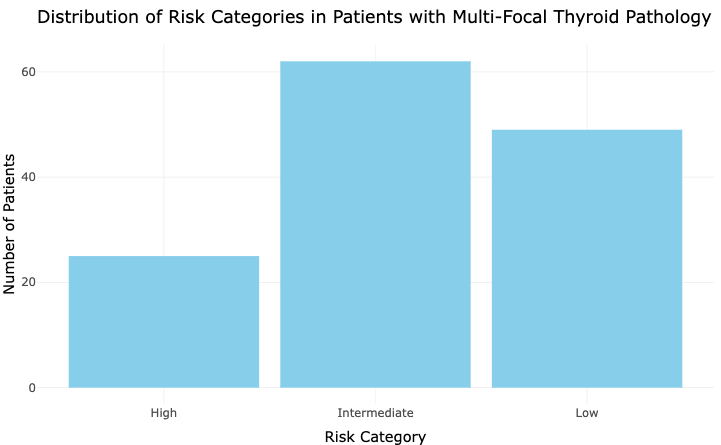
\includegraphics[width=1.1\textwidth]{risk vs multi.png}  
        \caption{Distribution of Risk categories with Multi-Focal Pathology}
            \label{fig:example}
       \vspace{0.5cm}
    \end{figure}

The distribution of risk categories in the given bar chart among the patients with multi-focal thyroid pathology would indicate that by far, the highest number of the patients falls into the category of an intermediate risk category; therefore, though serious, it most often presents with such a level of risk which may still enable rather effective management and intervention. Next comes the low-risk category, entailing a great number of patients, which shows that the discovery of multi-focal pathologies is rather early or naturally less aggressive in most instances. The high-risk category has the fewest patients, reflecting situations where the pathology probably has more serious consequences and requires heavier medical interventions. This distribution underlines the relevance of differentiated treatment strategies, considering the level of risk pertinent to each specific patient to obtain the best results.

    \newpage

 \item \textbf{Do certain risk categories correlate with specific pathology types in thyroid cancer?} \\
    E: pecific pathology types in thyroid cancer correlate with risk categories; papillary and follicular types are usually lower risk.
    
    \begin{figure}[h]
        \vspace{5pt}
        \centering
        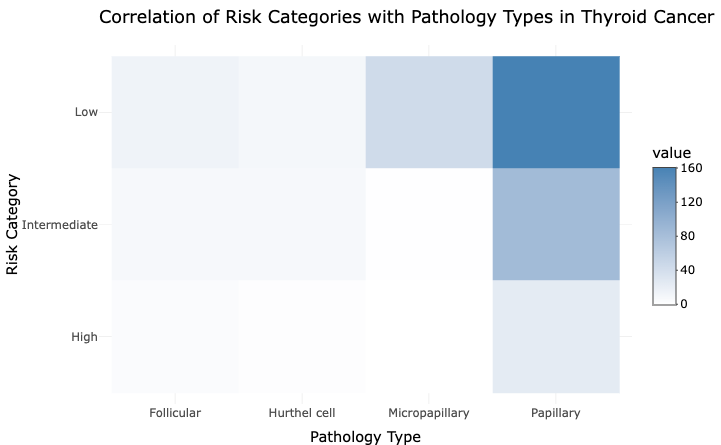
\includegraphics[width=1.1\textwidth]{risk vs path.png}  
        \caption{Correlation of Risk and Pathology Type}
            \label{fig:example}
       \vspace{0.5cm}
    \end{figure}

    The heatmap of risk category versus pathology type in thyroid cancer informs on how different pathological variants correspond with each other for varying levels of risk. Follicular pathology, which is known to be potentially clinically significant, predominantly features in the low and intermediate categories of risk, showing that it seldom escalates to a high-risk status to mostly have generally favorable cases upon early detection. The pathology of Hurthel cell mostly falls into the category of intermediate risk, reflecting its capability to present more serious challenges than the low-risk types but normally not progressing towards the most severe outcome. Micropapillary pathology, largely confined to the low-risk category, suggests its often indolent nature and good prognosis. In contrast, thyroid papillary carcinoma, the most common thyroid malignancy, is heavily weighted in the intermediate-risk category but also highly represented in the low-risk category, reflecting the generally less aggressive nature but variable prognosis based on individual case factors. The breakdown herein serves to underscore the clinical importance of risk stratification in thyroid cancer and reminds readers that pathology type may heavily influence both treatment approach and intensity of monitoring required.

\newpage

     \item \textbf{How does cancer stage relate to the age and gender of the patients?} \\
    E: Cancer stage often varies with age and gender, with older patients and males typically presenting at more advanced stages compared to younger individuals and females.
    \begin{figure}[h]
        \vspace{5pt}
        \centering
        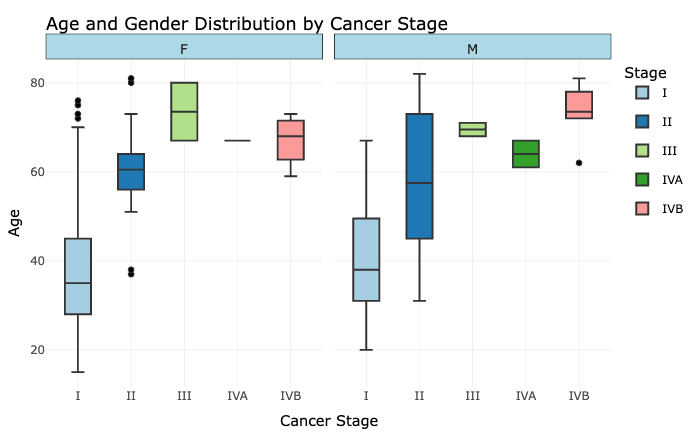
\includegraphics[width=1.1\textwidth]{age gender vs stage.png}  
        \caption{Distribution of Age and Gender across Cancer Stage}
            \label{fig:example}
       \vspace{0.5cm}
    \end{figure}

This boxplot shows the relationship between cancer stage, age, and gender for patients by showing clearly how these variables interact with each other. For females, it can be observed that the age range is great at Cancer Stage I, with the median approximately at 40 years, indicating that younger to middle-aged females are commonly diagnosed at this initial stage. The trend goes on up to stages II and III, showing a slight increase in median age, hence indicating that the majority of females are affected in these stages in middle age. The age range decreases as the stage goes to IV (IVA and IVB), showing a upward shift, especially in Stage IVB, which indicates that older females are likely to be diagnosed at this stage.

It means that the male distribution normally develops cancer at older ages compared to women. By Stage I, the age median of the male is higher, with an age distribution less diffused. With more advances in the stages of the disease, the distribution is wider, especially Stage IVA, where ages were spanned over a wide range, whereas Stage IVB concentrates around the older population. This trend again suggests the importance of targeted screening strategies, considering age and gender in order to optimize early detection and treatment outcomes.

\newpage

\item \textbf{How do gender and pathology type associate with the risk of thyroid cancer recurrence?} \\
E: Recurrence rates of thyroid cancer are expected to be higher in females compared to males, with certain aggressive pathology types also associated with increased recurrence risk.

 \begin{figure}[h]
        \vspace{5pt}
        \centering
        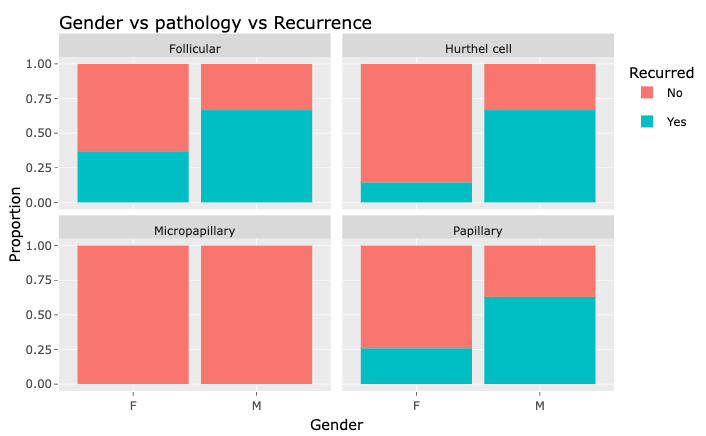
\includegraphics[width=1.1\textwidth]{gender vs path vs recc.png}  
        \caption{Gender vs pathology vs Recurrence}
            \label{fig:example}
       \vspace{0.5cm}
    \end{figure}

    This bar chart  gives the full picture of how gender and pathology type are associated with the risk of recurrence across pathology types: Follicular, Hurthel cell, Micropapillary, and Papillary. The rates of recurrence in Follicular and Hurthel cell pathologies are somewhat even between genders, though a little lower in females in the case of Follicular. In contrast, Micropapillary pathology exhibits a notably higher recurrence rate in males, suggesting a gender-specific vulnerability or perhaps different efficacies in treatment responses. Although generally the pathology of papillary is common to both sexes, men show a small but higher tendency toward recurrence. The visualization suggests that the kind of thyroid pathology and gender of the patient together play an important role in recurrence risks and thus require gender-informed approaches in clinical assessment and tailored treatment strategies for the optimization of outcomes.
    
\end{enumerate}

\newpage
\subsubsection{Treatment Outcomes}

\begin{enumerate}
    \item \textbf{What treatment responses are observed in different age groups? } \\
    E: Younger patients might respond better to treatments due to generally better health and fewer comorbidities.
    \begin{figure}[h]
        \vspace{5pt}
        \centering
        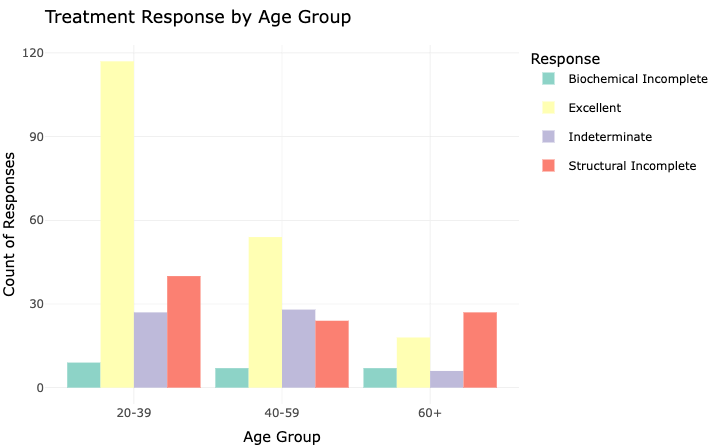
\includegraphics[width=1.15\textwidth]{tretament by age.png}  
        \caption{Treatment outcome by Age group}
            \label{fig:example}
       \vspace{0.2cm}
    \end{figure}

    The above bar chart presents treatment responses among subjects for the age groups of 20-39, 40-59, and 60+ for four categories of Biochemical Incomplete, Excellent, Indeterminate, and Structural Incomplete. Treatment responses in the younger patients were essentially "Excellent," infrequent "Biochemical Incomplete" and "Indeterminate," and the "Structural Incomplete" being almost nil for better recovery rates in this demographic category. The response pattern in the middle age category 40-59 is increasingly diverse, with a definite increase in "Biochemical Incomplete" responses, indicating some residual activity of their disease post-treatment. There is also "Indeterminate" and "Structural Incomplete" responses that may show more complicated health scenarios maybe because of older age. 
    
    Older patients do represent all types of responses, with a slight trend toward having fewer "Excellent" responses and higher incomplete responses, which points out some of the challenges in achieving optimal outcomes with therapy in this age group--possibly due to age-related physiological changes and higher susceptibility to complications. This trend also puts further emphasis on the place of age consideration in treatment planning and follow-up strategy for optimum health outcome at each stage of life.

\newpage
    
    \item \textbf{Does Gender  influence treatment outcomes?}\\ 
 E:It’s expected that male patients  may have less favorable treatment outcomes, as studies often indicate that  certain biological factors in males can lead to slower recovery and increased risk of complications compared to females .

   \begin{figure}[h]
        \vspace{5pt}
        \centering
        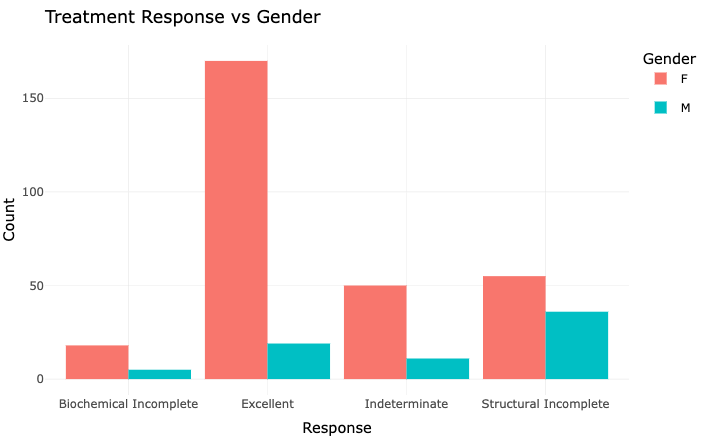
\includegraphics[width=1\textwidth]{treatment vs gender.png}  
        \caption{Treatment Response by Gender}
            \label{fig:example}
       \vspace{0.5cm}
    \end{figure}

The bar chart compares treatment responses between genders graphically; clear patterns are present among the male and female responses to therapy. The females outnumber the males by a great margin in the category "Excellent" response, hence suggesting that females have better overall treatment outcomes. This may suggest, first, either biological differences in disease pathology between genders or variations in how treatments are administered or received.

In contrast, the "Biochemical Incomplete" and "Structural Incomplete" categories have a slight male predilection over females, which could imply a higher residual or more resistant disease in males post-treatment. The "Indeterminate" response is relatively equally distributed between both genders; this would imply that uncertainty in the outcomes of treatment does not necessarily favor one gender over another. This may indicate that gender is a predicting factor for treatment response, as females generally tend to show better response rates in terms of complete response, though males might have a slightly greater tendency toward incomplete responses. In any case, this signals the importance of gender-specific consideration in treatment planning and follow-up.

\newpage

\item \textbf{Does Treatment Response Affect Recurrence of Thyroid Cancer?}\\ 
 E:Treatment responses are expected to influence the recurrence of thyroid cancer, with positive responses generally leading to lower recurrence rates compared to higher rates. 

\begin{figure}[h]
        \vspace{5pt}
        \centering
        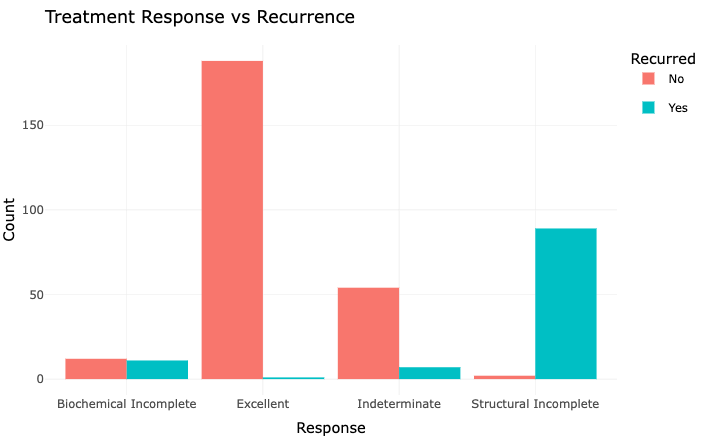
\includegraphics[width=1.1\textwidth]{response vs recurrence.png}  
        \caption{Treatment Response vs Recurrence}
            \label{fig:example}
       \vspace{0.5cm}
    \end{figure}

    The bar graph on the relationship of treatment response to recurrence in thyroid cancer clearly shows that the outcome of initial treatment has much bearing on recurrence rates. The recurrences are by far fewer in patients who obtain an "Excellent" response, which goes to show that successful initial treatment drastically reduces the likelihood of the disease returning. Whereas "Biochemical Incomplete" and "Structural Incomplete" responses have considerably higher recurrence rates, it would seem that incomplete eradication of cancer markers or residual structural disease presence represent high risks for recurrence. The "Indeterminate" response grade, though associated with fewer recurrences than incomplete responses, still carries some risk due to uncertainty in treatment outcomes. Overall, the findings stress the importance of a complete and effective initial response in treatments, as this will minimize recurrence risks of thyroid cancer and bring into focus precise and aggressive management strategies in cases with less-than-excellent initial responses.

\newpage
    
    \item \textbf{How does the average treatment response vary by cancer stage when considering different smoking statuses among thyroid cancer patients?}\\ 
 E:Average treatment responses are expected to vary by cancer stage and smoking status, with non-smokers generally exhibiting higher responses across all stages compared to smokers. Additionally, earlier stages of cancer typically demonstrate better treatment responses than advanced stages. 

\begin{figure}[h]
        \vspace{5pt}
        \centering
        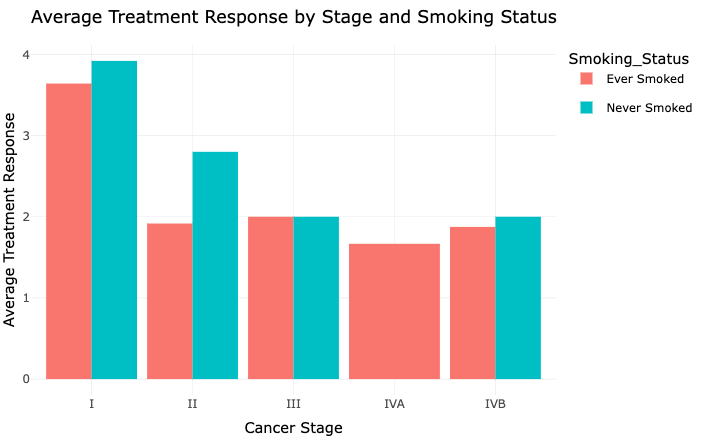
\includegraphics[width=1.1\textwidth]{average.png}  
        \caption{Treatment Response by Stage and Smoking status}
            \label{fig:example}
       \vspace{0.5cm}
    \end{figure}    
    

The bar chart of average treatment responses in thyroid cancer at different stages, differentiated by smoking status, depicts that early-stage cancer or Stage I responds well to treatment irrespective of the smoking background and hence reflects high treatment effectiveness for both smokers and non-smokers. But in Stage II and III, the drop is much more pronounced for those who have smoked, which might mean that smoking can indeed compromise treatment efficacy in mid-stage cancer. In the advanced IVA and IVB stages, the treatment response between smokers and non-smokers once more converges, albeit at levels lower than in previous stages. This would mean that at the intermediate stages, while treatment outcomes were poorer for smokers, in a case of advanced cancer, the gravity somewhat reduces the differential effects of smoking, reflecting complexity in the interaction of lifestyle variables and cancer progression.

\newpage


\item \textbf{What relationships exist between treatment outcomes and thyroid function categories?} \\
E: Treatment outcomes are expected to be more favorable in patients with normal thyroid function compared to those with hypothyroidism or hyperthyroidism, as well-controlled thyroid levels are linked to better responses and fewer complications.

 \begin{figure}[h]
        \vspace{5pt}
        \centering
        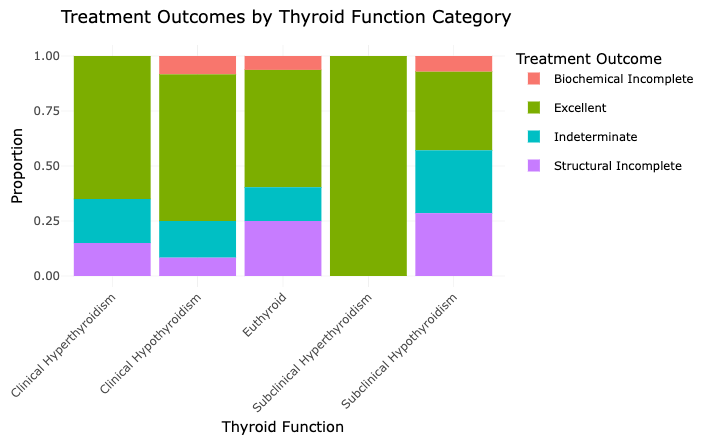
\includegraphics[width=1\textwidth]{treatment vs throif.png}  
        \caption{Treatment Response by thyroid functin}
            \label{fig:example}
       \vspace{0.3cm}
    \end{figure}

The stacked bar plot of treatment outcome by thyroid function status reflects a different effect of treatment. Notably, for both overt clinical thyroid dysfunctions-high and hypothyroidism-and for the euthyroid state, the "Excellent" category is higher in absolute levels, making it a general hypothesis that treatments work particularly well when the dysfunction of the thyroid is clear or not present. By contrast, the subclinical conditions are those that present milder and often less symptomatic forms of thyroid dysfunction, revealing a greater share of "Indeterminate" outcomes. This pattern shows that subtler manifestations of thyroid dysfunction in subclinical states might perplex the effectiveness of treatments and predictability of outcomes. Moreover, the presence of "Biochemical Incomplete" and "Structural Incomplete" responses in all categories points out the difficulty of the comprehensive response to thyroid treatment and makes the treatment highly individualized with regard to the degree and type of thyroid dysfunction for better therapeutic success and prognosis of the patient.

\newpage



\end{enumerate}


\newpage

\section{Summary}
This was a comprehensive study in which advanced data visualization techniques were used to explain complex relations among demographic factors, lifestyle influences, clinical features, and treatment outcomes in thyroid diseases. Based on extensive analysis of the large dataset, this study made a number of important observations regarding the progress and management of thyroid conditions.

\vspace{0.4cm}
\textbf{Key Observations}: 
\begin{itemize}


    
\item \textbf{Demographic Analysis}: The findings have indeed confirmed thyroid diseases to affect mainly females and also to be more common in young and middle-aged adults. It would, therefore, imply that targeted screening and prevention measures should be developed to ensure effective thyroid conditions' management in these groups.

\item \textbf{Lifestyle and History Factors}: Data on life factors such as smoking and radiotherapy revealed their explicit relation to the extent of pathology of the thyroid gland. Patients with a history of smoking or radiotherapy came out with more advanced stages of the disease upon diagnosis; hence, proving the mentioned influences significantly in thyroid health.

\item \textbf{Medical Analysis}:The medical analyses also indicated that the thyroid stage is closely related to cancer stage, with euthyroid patients being diagnosed while in their early stages of this disease. This suggests that assessment of thyroid function may be important in early detection and intervention in thyroid cancer.

\item \textbf{Clinical Feature}:In the study, clinical features associated with the disease, such as adenopathy, were highly associated with the cancer staging and recurrence rates of the thyroid. In general, patients presenting with adenopathy showed advanced diseases and had higher recurrence rates, thereby underlining the use of clinical features in assessing disease severity and prognosis.

\item \textbf{Cancer-specific Analysis}: The study showed how demographic variables like age and gender impact the distribution of TNM staging in thyroid cancer patients. Generally speaking, younger and female participants usually presented with an earlier stage of cancer that underlined demographic factors influencing disease outcomes.

\item \textbf{Treatment Outcomes}: Response to treatment varied importantly according to different demographic groups. Better outcomes were seen among younger people and nonsmokers. Moreover, the type of thyroid dysfunction had an important influence on the effectiveness of treatment: among euthyroid patients, treatment protocols were more likely to be successful.

\end{itemize}

\newpage

\section{Future Work}
Further research can be done along various lines in the extension of findings from the present study:

\begin{itemize}
    
    \item \textbf{Longitudinal Studies}: Longitudinal studies may actually enable observation of the disease over time and treatment effectiveness within the same cohort. This may yield temporal patterns and long-term outcomes which may not be evident within cross-sectional studies.
    \item \textbf{Larger Datasets}:Larger datasets from more diverse populations would carry more validity of the initial findings of this study and their generalization in other populations. This could include an international dataset comprising patient data assessing geographic and ethnic differences in presentation and treatment outcomes of thyroid disease.
    \item \textbf{Application of Machine Learning}: Application of machine learning may show predictive values of patient outcomes as complex interactions of studied variables. Predictive modeling may allow the early identification of people at risk and offer personalized treatment programs.
    \item \textbf{Genetic and Molecular Studies}: Genetic and molecular studies in thyroid disorders may attain better understanding of biological underpinning with the possible application of targeted therapies.
\item \textbf{Assessment of New and Emerging Therapies}: The evaluation of the impact new and emerging therapies will make on thyroid disease outcomes is very important. This would relate not only to new pharmacological interventions but also to novel therapeutic approaches, such as precision medicine and personalized treatment plans based on a genetic profile.
\end{itemize}



\newpage


\begin{thebibliography}{99}
  \bibitem[Arthur and Beckett, 1999]{Arthur&Beckett}
   Arthur, J.R. and Beckett, G.J., 1999. Thyroid function. British Medical Bulletin, 55(3), pp.658-668. doi:10.1258/0007142991902538.

    \bibitem[Bauer et al., 2013]{Bauer}
    Bauer, M., Goetz, T., Glenn, T. and Whybrow, P.C., 2013. Gender differences in thyroid system function: relevance to bipolar disorder and its treatment. Bipolar Disorders, 16(1), pp.58-71. doi:10.1111/bdi.12150.
    
    \bibitem[Cabanillas et al., 2016]{cabanillas2016}
    Cabanillas, M.E., McFadden, D.G. and Durante, C., 2016. Thyroid cancer. The Lancet, 388(10061), pp.2783-2795. doi:10.1016/s0140-6736(16)30172-6.

    \bibitem[Cooper et al., 2009]{Cooper}
    Cooper, D.S., Doherty, G.M., Haugen, B.R., Kloos, R.T., Lee, S.L., Mandel, S.J., Mazzaferri, E.L., McIver, B., Sherman, S.I. and Tuttle, R.M., 2009. Revised American thyroid association management guidelines for patients with thyroid nodules and differentiated thyroid cancer. Thyroid, 19(11), pp.1167-1214. doi:10.1089/thy.2009.0110.
    
    \bibitem[Durante et al., 2018]{Durante}
    Durante, C., Grani, G., Lamartina, L., Filetti, S., Mandel, S.J. and Cooper, D.S., 2018. The diagnosis and management of thyroid nodules. JAMA, 319(9), pp.914-924. doi:10.1001/jama.2018.0898.

    \bibitem[Vanderpump, 2011]{Vanderpump}
    Vanderpump, M.P., 2011. The epidemiology of thyroid disease. British Medical Bulletin, 99(1), pp.39-51. doi:10.1093/bmb/ldr030.
\end{thebibliography}



\end{document}